\documentclass[twoside,leqno]{article}

% Comment out the line below if using A4 paper size
\usepackage[letterpaper]{geometry}

\usepackage{siamproceedings}

\usepackage[T1]{fontenc}
\usepackage{amsmath,amssymb,amsfonts}
\usepackage{graphicx}
\usepackage{epstopdf}
\usepackage{enumitem}

\usepackage[title]{appendix}
\usepackage{listings}
\usepackage{algorithm}
\usepackage{algorithmicx}
\usepackage{algpseudocode}
\usepackage{tikz}
\usepackage{url}
\usepackage{adjustbox}
\usepackage{textcomp}
\usepackage{booktabs}
\usepackage{hyperref}
\usepackage{tcolorbox}
\usetikzlibrary{arrows.meta,backgrounds}
\usetikzlibrary{arrows,automata}
\usetikzlibrary{arrows.meta,positioning,decorations.pathreplacing}

\lstset{
    basicstyle=\ttfamily,
    breaklines=true,
    frame=single,
    language=HTML,
    showstringspaces=false,
    commentstyle=\color{gray},
    keywordstyle=\color{blue},
    stringstyle=\color{red},
    upquote=true
}

\newtcolorbox{stoppingcondition}[1][]{
  colback=cyan!10!white,
  colframe=cyan!75!black,
  fonttitle=\bfseries\large,
  title=#1,
  boxrule=1.5pt,
  left=12pt,
  right=12pt,
  top=10pt,
  bottom=10pt
}

%% ---- orbit colours (same pastel family as the unfolding figure) ----
\tikzset{
  vtx/.style   ={circle,draw=black!70,line width=0.5pt,minimum size=7mm,
                 inner sep=0pt,font=\small},
  orbA/.style  ={vtx,fill=blue!12},
  orbB/.style  ={vtx,fill=orange!20},
  orbC/.style  ={vtx,fill=green!16},
  orbD/.style  ={vtx,fill=violet!16},
  orbE/.style  ={vtx,fill=yellow!35},
  ed/.style    ={->,draw=black!70,line width=0.6pt},
  edbreak/.style ={->,draw=red!65!black,line width=0.9pt},
  ann/.style     ={font=\footnotesize,inner sep=1.5pt},
}


\ifpdf
  \DeclareGraphicsExtensions{.eps,.pdf,.png,.jpg}
\else
  \DeclareGraphicsExtensions{.eps}
\fi

% Add a serial/Oxford comma by default.
\newcommand{\creflastconjunction}{, and~}

% Used for creating new theorem and remark environments
\newsiamremark{remark}{Remark}
\newsiamremark{hypothesis}{Hypothesis}
\crefname{hypothesis}{Hypothesis}{Hypotheses}
\newsiamthm{claim}{Claim}
\newsiamthm{prop}{Proposition}
\newsiamthm{cor}{Corollary}
\newsiamremark{defn}{Definition}
\newsiamremark{exmp}{Example}

\usepackage{amsopn}
\DeclareMathOperator{\diag}{diag}
\DeclareMathOperator{\Aut}{Aut}
\DeclareMathOperator{\Orb}{Orb}

%% ---- notation ----
\newcommand{\HG}{\mathcal{H}_{G}}
\newcommand{\HN}{\mathcal{H}_{N}}
\newcommand{\HL}{\mathcal{H}_{L}}
\newcommand{\HB}{\mathcal{H}_{B}}
\newcommand{\HO}{\mathcal{H}_{O}}
\newcommand{\HM}{\mathcal{H}_{M}}
\newcommand{\enc}{\mathrm{enc}}
\newcommand{\canon}{\mathrm{canon}}
\newcommand{\Unf}{\mathcal{T}}
\newcommand{\Reach}{R}
\newcommand{\mset}[1]{\{\!\!\{#1\}\!\!\}}
\newcommand{\iso}{\cong}


\begin{document}

%
\newcommand\relatedversion{}
%\renewcommand\relatedversion{\thanks{The full version of the paper can be accessed at \protect\url{https://arxiv.org/abs/0000.00000}}} % Replace URL with link to full paper or comment out this line

\title{\Large Directed Graph Hashing\relatedversion}
    \author{Caleb Helbling\thanks{Draper (\email{chelbling@draper.com}).}}

\date{}

\maketitle

% Default Copyright Statement
\fancyfoot[R]{\scriptsize{Copyright \textcopyright\ 20XX by SIAM\\
Unauthorized reproduction of this article is prohibited}}

%\fancyfoot[R]{\scriptsize{Copyright \textcopyright\ 20XX\\
%Copyright for this paper is retained by authors}}

%\fancyfoot[R]{\scriptsize{Copyright \textcopyright\ 20XX\\
%Copyright retained by principal author's organization}}

\begin{abstract}
  We present methods, with correctness proofs, for hashing node-labeled directed graphs and the individual nodes within them. We distinguish between hashing based on the \emph{global} structure of a graph, where equal hashes correspond to isomorphism and automorphism orbits, and hashing based on \emph{local} observations obtained by traversing the graph along its edges, where equal hashes correspond to isomorphic (possibly infinite) unfoldings or, in a variant, to bisimilarity. For graphs whose outgoing edges are ordered we give linear-time node hashes and a quadratic-time canonization of strongly connected graphs, and we combine these ingredients into a Merkle-style hash that recurses over the condensation of a graph, for which we characterize exactly which nodes receive equal hashes. We also show that hashing nodes by the language of their walks is PSPACE-hard. Structural hashing of trees is ubiquitous in blockchains, version control, and content-addressed storage; by contrast, hashing of cyclic directed graphs has received comparatively little systematic treatment. A reference implementation is validated against brute-force equivalence checks, and we report its running time on random digraphs.
\end{abstract}

\section{Introduction}\label{sec:introduction}

Hashing functions are fundamental building blocks in the modern software stack that have seen widespread use in data storage and retrieval, digital fingerprinting, checksum and cryptographic applications. Traditionally, hash functions take as input bit strings of arbitrary length and return a bit string of a fixed size $\mathcal{H} : \{0,1\}^* \rightarrow \{0,1\}^n$. Good hashing functions should be fast to compute, minimize the chance of duplication of output values, and produce large changes in output for small changes in input. Many bit string hashing functions have been created over the years, including well known algorithms such as MD5 \cite{md5}, SHA-2 \cite{sha2}, and SHA-3 \cite{sha3}.

\begin{algorithm}
\caption{Recursive Merkle-tree Hashing of Ordered Binary Tree}
\[
\text{mh}(n) =
\begin{cases}
    \mathcal{H}(n.\text{label}) & n \text{ is a leaf} \\
    \mathcal{H}(n.\text{label} \circ \text{mh}(n.\text{left}) \circ \text{mh}(n.\text{right})) & \text{otherwise}
\end{cases}
\]
\label{alg:merklehashing}
\end{algorithm}

Hashing functions can be extended to trees via a simple extension of Merkle hashing \cite{merkle1987digital}. In Merkle tree hashing, the hash of a node is computed by hashing the concatenation of the node's label with the recursive hash of the node's children. Algorithm \ref{alg:merklehashing} gives a simple recursive implementation of Merkle tree hashing for ordered binary trees. This particular variation of Merkle hashing has seen use in many applications, including cryptocurrency \cite{bitcoin}, version control systems \cite{git}, and distributed hypertext document storage systems \cite{ipfs}. For \emph{unordered} trees, replacing the sequence of child hashes by a sorted multiset of child hashes yields a hash that is invariant under tree isomorphism, in the spirit of the classical Aho--Hopcroft--Ullman tree isomorphism algorithm \cite{aho1974design}.

Extending hashing to node-labeled directed graphs is non-trivial due to the presence of cycles: the recursion of Algorithm~\ref{alg:merklehashing} no longer terminates. Indeed, the design space for hashing digraphs is surprisingly broad and depends on use case objectives. In this paper we focus on the following approaches, which we think are the most useful for practical applications:

\begin{itemize}
  \item \textbf{Global Hashing} (Section \ref{sec:global-graph-hashing}) --- for use cases where the \textit{global} structure of the digraph is of importance. Two graphs hash equally if and only if they are isomorphic, and two nodes hash equally if and only if some isomorphism of their graphs maps one onto the other; in particular, nodes in the same automorphism orbit hash equally.
  \item \textbf{Local Hashing} (Section \ref{sec:local-graph-hashing}) --- for use cases where observers can only observe \textit{local} information by traversing from a node to a neighbor on an outgoing edge. Two nodes hash equally if and only if the (potentially infinite) trees obtained by unfolding the graph from them are isomorphic. We also give a variant for bisimilarity, and show that hashing by the language of walks is PSPACE-hard. Local hashing has many commonalities with bisimulation and co-inductive representations of finite directed graphs \cite{bisimulation_book,coinductive_graphs}.
  \item \textbf{Ordered Outgoing Edges} (Section \ref{sec:outgoing-ordered-edge-graphs}) --- in many practical applications the outgoing edges from a node are ordered. We use this additional structure to obtain linear-time node hashes and a quadratic-time canonization of strongly connected graphs.
  \item \textbf{Merkle Graph Hashing} (Section \ref{sec:merkle-graph-hashing}) --- for use cases where graphs are hashed recursively, or are built up over time. We hash strongly connected components individually, then recurse over the acyclic condensation graph. We characterize precisely which nodes receive equal hashes: the resulting equivalence lies strictly between rooted isomorphism and unfolding equivalence.
\end{itemize}

One common theme throughout this paper is reliance on conversion of graphs to \textit{canonical form}. If two graphs (or nodes within them) can be converted to a canonical form, we can serialize the canonical form and pass it through an ordinary string hashing function. We distinguish carefully between the hash of an entire graph and the hash of a specific node within a graph. Our general strategy for computing the hash of a specific node is to combine the overall graph hash with the node's position in canonical order, taking care that this position accounts for any symmetry present in the graph (two nodes may be identical modulo automorphism).

\paragraph{Contributions.} Each hashing scheme comes with an exact characterization of hash equality (Theorems \ref{thm:digraphhashcorrect}, \ref{thm:digraphnodehashcorrect}, \ref{thm:localhashcorrect}, \ref{thm:bisimhash}, \ref{thm:orderedhash}, \ref{thm:scc-ordered} and \ref{thm:merkle}), stated relative to an idealized string hash (Section~\ref{sec:hash-model}). We identify and prove the \emph{local stabilization} property that makes color-refinement colors usable as a canonical order (Lemma~\ref{lem:local-injective}), prove PSPACE-hardness of hashing walk languages (Proposition~\ref{prop:pspace}), and position the Merkle scheme relative to the other equivalences (Proposition~\ref{prop:merkle-position}). A reference implementation is validated against brute-force checks and benchmarked in Section~\ref{sec:experiments}.

\section{Preliminaries}
\label{sec:preliminaries}

\begin{figure*}[!b]
\centering
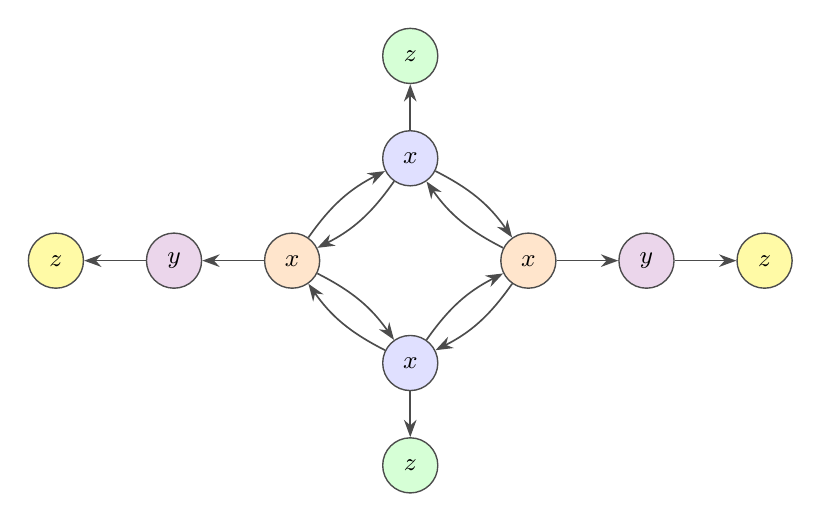
\begin{tikzpicture}[
  >={Stealth[length=2.2mm,width=1.6mm]},
  x=1cm, y=1cm,
]

%% ---------------- vertices ----------------
%% letters are node LABELS; fill colours are ORBITS
\node[orbC] (e) at ( 0.0, 2.6) {$z$};
\node[orbA] (a) at ( 0.0, 1.3) {$x$};
\node[orbB] (b) at (-1.5, 0.0) {$x$};
\node[orbB] (c) at ( 1.5, 0.0) {$x$};
\node[orbA] (d) at ( 0.0,-1.3) {$x$};
\node[orbC] (f) at ( 0.0,-2.6) {$z$};

\node[orbD] (g) at ( 3.0, 0.0) {$y$};
\node[orbE] (h) at ( 4.5, 0.0) {$z$};
\node[orbD] (i) at (-3.0, 0.0) {$y$};
\node[orbE] (j) at (-4.5, 0.0) {$z$};

%% ---------------- edges ----------------
%% bidirectional edges of the central diamond: one arc per direction
\foreach \u/\v in {a/b, a/c, b/d, c/d}{
  \draw[ed] (\u) to[bend left=14] (\v);
  \draw[ed] (\v) to[bend left=14] (\u);
}

%% pendant edges
\draw[ed] (a) -- (e);
\draw[ed] (d) -- (f);
\draw[ed] (c) -- (g);
\draw[ed] (g) -- (h);
\draw[ed] (b) -- (i);
\draw[ed] (i) -- (j);

\end{tikzpicture}
\caption{A directed graph with three node labels ($x$, $y$, $z$, shown as letters) and five automorphism orbits (shown by fill colour). Its automorphism group has order four and is generated by the two reflections of the drawing (their product is the rotation by $180^\circ$). Equal labels do not imply equal orbits: the four $x$-labelled nodes of the central diamond fall into two orbits, and the four $z$-labelled sinks fall into two orbits, because an $x$-node's pendant neighbour is a sink in one case and has a successor in the other.}
\label{fig:orbitexample}
\end{figure*}

\subsection{Labeled digraphs and symmetry.}
A \emph{labeled digraph} is a triple $G=(V,E,L)$ where $V$ is a finite vertex set, $E \subseteq V \times V$ is the edge set (self-loops are allowed), and $L$ maps vertices to labels drawn from a set of strings. In Section~\ref{sec:local-graph-hashing} we also use \emph{labeled multidigraphs} $G=(V,\mu,L)$, where $\mu : V\times V \to \mathbb{N}$ gives edge multiplicities; a digraph is the special case $\mu(u,v)=[(u,v)\in E]$. We write $\mathrm{succ}(u)$ for the multiset of successors of $u$ (with $v$ occurring $\mu(u,v)$ times), and $\Reach(u)$ for the set of vertices reachable from $u$ (including $u$). A set $S \subseteq V$ is \emph{forward-closed} if every successor of a vertex of $S$ lies in $S$; each $\Reach(u)$ is forward-closed, and so is $V$.

An \emph{isomorphism} $\phi : G_1 \to G_2$ is a bijection $V_1 \to V_2$ with $L_2(\phi(u)) = L_1(u)$ and $\mu_2(\phi(u),\phi(v)) = \mu_1(u,v)$ for all $u,v$; we write $G_1 \iso G_2$. A \emph{rooted isomorphism} $(G_1,v_1) \iso (G_2,v_2)$ is an isomorphism with $\phi(v_1)=v_2$. An \emph{automorphism} is an isomorphism $G\to G$; the automorphisms form the group
\[
\Aut(G) = \{ \sigma : V \to V \text{ bijective} \mid L(\sigma(u)) = L(u),\ (u, v) \in E \leftrightarrow (\sigma(u), \sigma(v)) \in E\}.
\]
Informally, the automorphism group gives all of the ways that $G$ is symmetrical. The \emph{orbit} of a vertex is the set of vertices it can be mapped to by automorphisms,
\[
\Orb(G, v) = \{\sigma(v) \mid \sigma \in \Aut(G)\},
\]
and the orbits partition $V$. Figure~\ref{fig:orbitexample} gives an example. Note that $v_1$ and $v_2$ lie in the same orbit of $G$ if and only if $(G,v_1)\iso(G,v_2)$.

\subsection{Canonical forms.}
Fix a canonical labeling procedure (for example nauty/Traces \cite{nauty,mckay2014practical}, bliss \cite{bliss}, or saucy \cite{saucy}, all of which support vertex labels). Given $G$ with $|V|=n$ it returns a bijection $\rho_G : V \to \{0,\dots,n-1\}$ such that the relabeled graph $\canon(G) = \rho_G(G)$ satisfies
\[
\canon(G_1) = \canon(G_2) \iff G_1 \iso G_2 .
\]
By construction $\rho_G$ is an isomorphism $G\to\canon(G)$. It is determined only up to automorphisms: if $\rho$ is a canonical labeling then so is $\rho\circ\sigma$ for every $\sigma \in \Aut(G)$, and no canonical labeling procedure can prefer one of these over another. This is precisely why node hashes must be defined through orbits rather than through canonical indices alone.

\begin{figure}
  \centering
  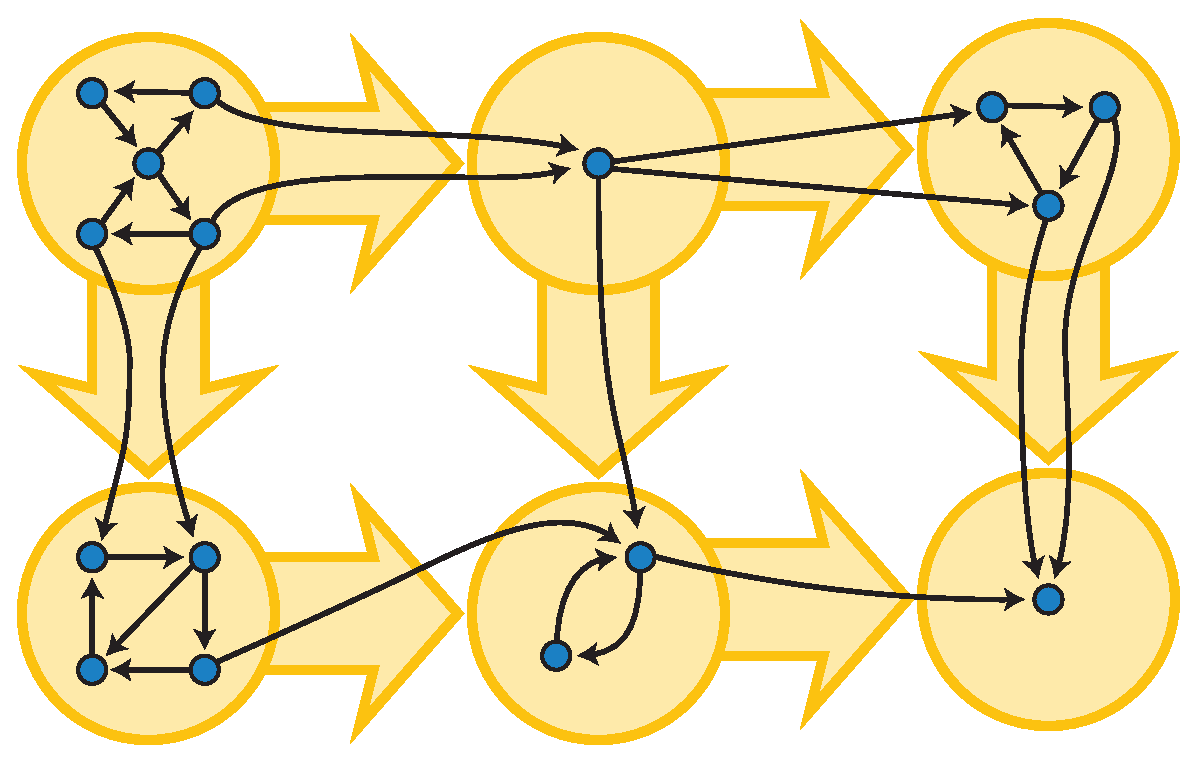
\includegraphics[width=0.5\linewidth]{Fig2.eps}
  \caption{Each yellow node contains a strongly connected component of a graph. When each strongly connected component is contracted into a single node, the yellow condensation graph is formed. Since the condensation graph is acyclic, it can be recursed over. Public domain figure courtesy of David Eppstein.\protect\footnotemark}
  \label{fig:condensation}
\end{figure}

\footnotetext{\url{https://commons.wikimedia.org/wiki/File:Graph_Condensation.svg}}

\subsection{Strongly connected components.}
A \textit{strongly connected component} (SCC) of a digraph is a maximal set of vertices such that there is a path between any two of them. The \textit{condensation graph} is formed by contracting each SCC into a single node; it is acyclic, and all SCCs together with the condensation can be computed in linear time \cite{tarjan1972depth}. The \emph{height} of an SCC is the number of edges on a longest path starting from it in the condensation. Figure \ref{fig:condensation} shows an example.

\subsection{The hashing model.}
\label{sec:hash-model}
All of our schemes serialize a finite structure and apply a string hash $\mathcal{H}$. We assume a serialization $\enc(\cdot)$ of nested tuples, lists, integers and strings that is \emph{injective} (for example, prefixing every item with a type tag and its length, so that labels containing delimiter characters cannot cause ambiguity), and we encode a multiset as the sorted list of its elements. Since $\mathcal{H}$ maps into a finite set it cannot be injective, so we state our theorems in the following sense.

\begin{defn}[Correctness up to collisions]
\label{def:correct}
A hash $h$ \emph{realizes} an equivalence relation $\sim$ if (i) $x \sim y$ implies $h(x)=h(y)$, and (ii) whenever $h(x) = h(y)$ but $x \not\sim y$, the computations of $h(x)$ and $h(y)$ contain two distinct strings $s \ne s'$ with $\mathcal{H}(s) = \mathcal{H}(s')$.
\end{defn}

Condition (ii) says that a failure of the ``only if'' direction exhibits an explicit collision of $\mathcal{H}$, which is believed infeasible for SHA-2 or SHA-3. Equivalently, every statement ``$h(x)=h(y)$ if and only if $x\sim y$'' below is proved under the idealization that $\mathcal{H}$ is injective, and each proof of the ``only if'' direction uses injectivity only by comparing two strings whose hashes are equal. For readability we say ``assuming $\mathcal{H}$ is injective'' in the proofs.

\section{Global Graph Hashing}
\label{sec:global-graph-hashing}

\begin{algorithm}[b]
    \caption{Global Digraph Hash}\label{digraphhash}
    \begin{algorithmic}[1]
    \Function{$\HG$}{$G=(V,E,L)$}
        \State $\rho \gets$ \textproc{canonize}($G$) \Comment{canonical labeling $\rho : V \to \{0,\dots,|V|-1\}$}
        \State adj\_list $\gets$ \textproc{sort}($[(\rho(u), \rho(v)) \mid (u,v) \in E]$)
        \State labels $\gets$ $[L(\rho^{-1}(i))$ \textbf{for} $i = 0, \dots, |V|-1]$
        \State \Return $\mathcal{H}$($\enc$((labels, adj\_list)))
    \EndFunction
    \end{algorithmic}
\end{algorithm}

In global graph hashing, we would like our computed hash values to be unique modulo graph isomorphism: $\HG(G_1)=\HG(G_2)$ if and only if $G_1 \iso G_2$. We canonize the input digraph and construct an adjacency list sorted in canonical order. The node labels (in canonical order) and the canonical adjacency list are then serialized and hashed using a string hashing function $\mathcal{H}$. Algorithm \ref{digraphhash} gives an implementation of this approach. Note that the pair (labels, adj\_list) is exactly an encoding of $\canon(G)$: the number of vertices is the length of the label list, so isolated vertices are accounted for.

\begin{theorem}[Correctness of the global graph hash]
\label{thm:digraphhashcorrect}
$\HG$ realizes graph isomorphism: assuming $\mathcal{H}$ is injective, $\HG(G_1)=\HG(G_2)$ if and only if $G_1 \iso G_2$.
\end{theorem}

\begin{proof}
($\Rightarrow$) If $\HG(G_1)=\HG(G_2)$, then by injectivity of $\mathcal{H}$ and $\enc$ the canonical label lists and adjacency lists coincide, i.e.\ $\canon(G_1)=\canon(G_2)$. Hence $G_1 \iso G_2$.

($\Leftarrow$) If $G_1 \iso G_2$ then $\canon(G_1)=\canon(G_2)$, so the label lists and sorted adjacency lists coincide, and so do their encodings and hashes.
\end{proof}

\paragraph{Complexity.} Since $\HG$ decides isomorphism of labeled digraphs (in the idealized model), computing it is at least as hard as graph isomorphism (GI). No polynomial-time algorithm for GI is known; the best known worst-case bound is quasipolynomial, both for isomorphism testing \cite{babai2016quasipolynomial} and for canonization \cite{babai2019canonical}. Practical canonization tools based on individualization and refinement \cite{nauty,mckay2014practical,bliss,saucy} are extremely fast on most inputs, but have exponential worst-case running time on specially constructed families. The same remarks apply to computing orbits, which Algorithm~\ref{alg:digraph-node-hash} below requires; tools such as nauty return the orbit partition as a by-product of canonization.

\begin{algorithm}[t]
    \caption{Global Digraph Node Hash}\label{alg:digraph-node-hash}
    \begin{algorithmic}[1]
    \Function{$\HN$}{$G$, $v$}
        \State $\rho \gets$ \textproc{canonize}($G$) \Comment{the same $\rho$ is used in the next line}
        \State g\_hash $\gets \HG(G)$ \Comment{computed from $\rho$ as in Algorithm~\ref{digraphhash}}
        \State orbit\_idx $\gets$ $\min\,\Orb(\canon(G), \rho(v))$
        \State \Return $\mathcal{H}$($\enc$((orbit\_idx, g\_hash)))
    \EndFunction
    \end{algorithmic}
\end{algorithm}

The algorithm for hashing nodes builds on the algorithm for hashing graphs. First, the graph is canonized and the hash of the canonical graph is computed using Algorithm \ref{digraphhash}. Then we compute the \emph{orbit index} of the input vertex: the smallest canonical index in the orbit of $\rho(v)$ in the canonical graph $\canon(G)$. (Equivalently, it is $\min\{\rho(u) \mid u \in \Orb(G,v)\}$, since $\rho$ maps orbits of $G$ onto orbits of $\canon(G)$.) The orbit index and the graph hash are then combined and passed through a string hashing function. Algorithm \ref{alg:digraph-node-hash} gives an implementation of this approach. The orbit index does not depend on which canonical labeling $\rho\circ\sigma$, $\sigma\in\Aut(G)$, the canonizer happens to return, since $\rho(\sigma(v))$ lies in the same orbit of $\canon(G)$ as $\rho(v)$.

\begin{theorem}[Correctness of the global node hash]
\label{thm:digraphnodehashcorrect}
$\HN$ realizes rooted isomorphism: assuming $\mathcal{H}$ is injective, $\HN(G_1, v_1)=\HN(G_2, v_2)$ if and only if there is an isomorphism $\phi : G_1 \to G_2$ with $\phi(v_1) = v_2$. In particular, two nodes of the same graph hash equally if and only if they lie in the same orbit.
\end{theorem}

\begin{proof}
Let $\rho_1,\rho_2$ be the canonical labelings of $G_1,G_2$.

($\Leftarrow$) Since $G_1\iso G_2$, $C:=\canon(G_1)=\canon(G_2)$ and $\HG(G_1)=\HG(G_2)$ by Theorem~\ref{thm:digraphhashcorrect}. The map $\alpha = \rho_2\circ\phi\circ\rho_1^{-1}$ is a composition of isomorphisms $C \to G_1 \to G_2 \to C$, hence $\alpha\in\Aut(C)$, and $\alpha(\rho_1(v_1)) = \rho_2(v_2)$. Thus $\rho_1(v_1)$ and $\rho_2(v_2)$ lie in the same orbit of $C$, so the orbit indices coincide, and so do the node hashes.

($\Rightarrow$) Equal node hashes imply, by injectivity, equal graph hashes and equal orbit indices. By Theorem~\ref{thm:digraphhashcorrect} (and its proof) $\canon(G_1)=\canon(G_2)=:C$. Two orbits of $C$ with the same minimum element are the same orbit, so there is $\alpha \in \Aut(C)$ with $\alpha(\rho_1(v_1)) = \rho_2(v_2)$. Then $\phi = \rho_2^{-1}\circ\alpha\circ\rho_1$ is an isomorphism $G_1 \to G_2$ with $\phi(v_1)=v_2$.
\end{proof}

\section{Local Graph Hashing}
\label{sec:local-graph-hashing}

\begin{figure*}[!b]
\centering
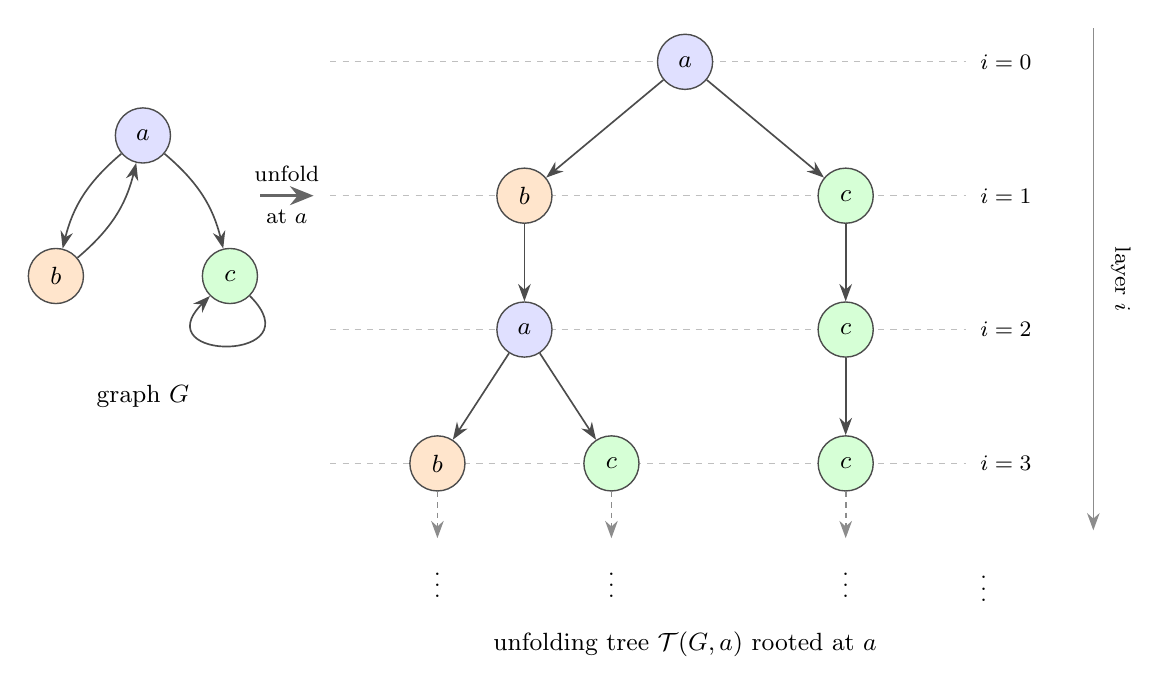
\begin{tikzpicture}[
  x=0.85cm, y=0.85cm,
  >={Stealth[length=2.2mm,width=1.6mm]},
  vtx/.style    ={circle,draw=black!70,line width=0.5pt,minimum size=7mm,
                  inner sep=0pt,font=\small},
  va/.style     ={vtx,fill=blue!12},
  vb/.style     ={vtx,fill=orange!20},
  vc/.style     ={vtx,fill=green!16},
  ed/.style     ={->,draw=black!70,line width=0.6pt},
  cont/.style   ={->,draw=black!45,line width=0.6pt,
                  dash pattern=on 2pt off 1.8pt,shorten >=2pt},
  layer/.style  ={draw=black!25,dash pattern=on 2.2pt off 2.2pt,line width=0.4pt},
  ilab/.style   ={font=\footnotesize,anchor=west,inner sep=2.5pt},
  dots/.style   ={font=\footnotesize,inner sep=1pt},
]
%% layer guides
\foreach \y/\i in {0/0, -2/1, -4/2, -6/3}{%
  \draw[layer] (-5.3,\y) -- (4.2,\y);
  \node[ilab] at (4.3,\y) {$i=\i$};
}
\node[ilab] at (4.3,-7.75) {$\vdots$};
\draw[->,draw=black!45,line width=0.5pt] (6.1,0.5) -- (6.1,-7.0)
      node[midway,right=1mm,font=\footnotesize,rotate=-90,anchor=south]
      {layer $i$};
%% left: the graph G (with cycles)
\begin{scope}[shift={(-8.1,-2.6)}]
  \node[va] (ga) at ( 0.0, 1.5) {$a$};
  \node[vb] (gb) at (-1.3,-0.6) {$b$};
  \node[vc] (gc) at ( 1.3,-0.6) {$c$};
  \draw[ed] (ga) to[bend right=18] (gb);   % a -> b
  \draw[ed] (gb) to[bend right=18] (ga);   % b -> a
  \draw[ed] (ga) to[bend left=18]  (gc);   % a -> c
  \draw[ed] (gc) to[out=-45,in=-135,looseness=6,
                    min distance=5mm] (gc);            % c -> c
  \node[font=\small] at (0,-2.4) {graph $G$};
\end{scope}
\draw[-{Stealth[length=3mm,width=2.4mm]},draw=black!60,line width=1pt]
      (-6.35,-2.0) -- (-5.55,-2.0)
      node[midway,above=0.5mm,font=\footnotesize]{unfold}
      node[midway,below=0.5mm,font=\footnotesize]{at $a$};
%% right: the unfolding
\node[va] (r)    at ( 0.0, 0) {$a$};
\node[vb] (b1)   at (-2.4,-2) {$b$};
\node[vc] (c1)   at ( 2.4,-2) {$c$};
\node[va] (a2)   at (-2.4,-4) {$a$};
\node[vc] (c2)   at ( 2.4,-4) {$c$};
\node[vb] (b3)   at (-3.7,-6) {$b$};
\node[vc] (c3)   at (-1.1,-6) {$c$};
\node[vc] (cc3)  at ( 2.4,-6) {$c$};
\draw[ed] (r)  -- (b1);
\draw[ed] (r)  -- (c1);
\draw[ed] (b1) -- (a2);
\draw[ed] (c1) -- (c2);
\draw[ed] (a2) -- (b3);
\draw[ed] (a2) -- (c3);
\draw[ed] (c2) -- (cc3);
\draw[cont] (b3)  -- (-3.7,-7.2);  \node[dots] at (-3.7,-7.7) {$\vdots$};
\draw[cont] (c3)  -- (-1.1,-7.2);  \node[dots] at (-1.1,-7.7) {$\vdots$};
\draw[cont] (cc3) -- ( 2.4,-7.2);  \node[dots] at ( 2.4,-7.7) {$\vdots$};
\node[font=\small] at (0,-8.7) {unfolding tree $\Unf(G, a)$ rooted at $a$};
\end{tikzpicture}
\caption{Unfolding of a directed graph with cycles. Starting from the root
$a$, every vertex is replaced by one copy per walk reaching it, so the cycle
$a\to b\to a$ and the self-loop $c\to c$ are unrolled into an infinite tree;
only the layers $i=0,\dots,3$ are drawn. Each tree node at layer $i$
corresponds to a walk of length $i$ from $a$ in $G$; colours indicate the
end vertex of the walk. The color $\lambda_i(a)$ is the (multiset) Merkle hash
of the truncation $\Unf_i(G,a)$ consisting of layers $0,\dots,i$.}
\label{fig:unfolding}
\end{figure*}

In comparison to the global hashing strategy which depends on the global structure of the graph, the local hashing strategy depends only on properties we can \textit{observe} by traversing the digraph forward along its edges. To make this concept precise, the hashes of two nodes should be equal if and only if their \textit{unfoldings} are isomorphic.

\subsection{Unfoldings.}
\begin{defn}[Unfolding]
%Let $G=(V,\mu,L)$ be a labeled multidigraph and $u\in V$. The \emph{unfolding} $\Unf(G,u)$ is the rooted, labeled, unordered tree whose nodes are the walks $w = (w_0, e_1, w_1, \dots, e_k, w_k)$ with $w_0 = u$, where $e_j \in \{1,\dots,\mu(w_{j-1},w_j)\}$ distinguishes parallel edges. The root is the walk $(u)$ of length $0$, the parent of a walk of length $k\ge 1$ is obtained by deleting its last step, and the label of $w$ is $L(w_k)$. The \emph{truncation} $\Unf_k(G,u)$ is the subtree of walks of length at most $k$.
Let $G=(V,\mu,L)$ be a labeled multidigraph and $u\in V$. The \emph{unfolding} $\Unf(G,u)$ is the rooted, labeled, unordered tree defined as follows. The nodes of $\Unf(G,u)$ are the walks in $G$ starting at $u$, i.e.\ sequences $w = (x_0, e_1, x_1, \dots, e_k, x_k)$ of vertices $x_j \in V$ of $G$ with $x_0 = u$ and $e_j \in \{1,\dots,\mu(x_{j-1},x_j)\}$ selecting one of the parallel edges from $x_{j-1}$ to $x_j$. Each walk, taken as a whole, is one tree node; the same vertex of $G$ can therefore occur in many tree nodes. The root is the walk $(u)$ of length $0$, the parent of a walk of length $k\ge 1$ is obtained by deleting its last step $(e_k, x_k)$, and the label of $w$ is $L(x_k)$, the label of the vertex at which the walk ends. The \emph{truncation} $\Unf_k(G,u)$ is the subtree of walks of length at most $k$.
\end{defn}

Isomorphism of rooted labeled unordered trees means a label-preserving bijection preserving the root and the parent relation. Two finite such trees are isomorphic if and only if the roots have equal labels and there is a bijection between the children of the two roots that maps each child subtree to an isomorphic child subtree. We use two elementary facts. First, the subtree of $\Unf(G,u)$ below a walk ending at $x$ is isomorphic to $\Unf(G,x)$. Second, the root of $\Unf(G,u)$ has exactly $\mu(u,x)$ children whose subtrees are copies of $\Unf(G,x)$, for each $x$. Unfoldings are infinite as soon as a cycle is reachable, but they are finitely branching. Figure \ref{fig:unfolding} shows an example.

\begin{lemma}[Truncations suffice]
\label{lem:truncation}
$\Unf(G_1,u)\iso\Unf(G_2,v)$ if and only if $\Unf_k(G_1,u)\iso\Unf_k(G_2,v)$ for every $k\ge 0$.
\end{lemma}
\begin{proof}
($\Rightarrow$) An isomorphism preserves depth, so it restricts to isomorphisms of the truncations.
($\Leftarrow$) Let $I_k$ be the set of isomorphisms $\Unf_k(G_1,u) \to \Unf_k(G_2,v)$. Each $I_k$ is finite (the trees are finite) and nonempty by assumption, and restriction maps $I_{k+1}$ into $I_k$. Let $J_k \subseteq I_k$ be the set of elements of $I_k$ that are restrictions of elements of $I_j$ for every $j > k$. Since the images of $I_j$ in $I_k$ form a decreasing chain of finite nonempty sets, $J_k$ is nonempty, and every element of $J_k$ is the restriction of an element of $J_{k+1}$. By K\H{o}nig's lemma \cite{konig1936theorie} (or simply by induction) there is a sequence $\phi_k \in J_k$ with $\phi_{k+1}$ extending $\phi_k$. Their union is an isomorphism $\Unf(G_1,u)\to\Unf(G_2,v)$.
\end{proof}

\subsection{Color refinement.}
Our strategy for local graph hashing uses a variant of color refinement \cite{weisfeiler1968reduction,Shervashidze2011-dt} along outgoing edges. The initial coloring is the hash of the node label, and each round combines a node's label with the multiset of its successors' colors (a multiset is serialized by sorting):
\begin{align}
  \lambda_0(u) &= \mathcal{H}(\enc(L(u))), \label{eq:coloring-init}\\
  \lambda_{i+1}(u) &= \mathcal{H}\big(\enc\big((L(u), \mset{\lambda_{i}(v) \mid v \in \mathrm{succ}(u)})\big)\big). \label{eq:coloring-step}
\end{align}
Note that the colors are defined for nodes of \emph{any} graph by the same formula, so colors of nodes in different graphs can be compared.

\begin{lemma}
\label{lem:colors-trunc}
Assuming $\mathcal{H}$ is injective, for nodes $u$ of $G_1$ and $v$ of $G_2$ and every $i \ge 0$: $\lambda_i(u)=\lambda_i(v)$ if and only if $\Unf_i(G_1,u)\iso\Unf_i(G_2,v)$. Consequently the colorings refine monotonically: $\lambda_{i+1}(u) = \lambda_{i+1}(v)$ implies $\lambda_i(u) = \lambda_i(v)$.
\end{lemma}
\begin{proof}
Induction on $i$. For $i=0$ both sides say $L_1(u)=L_2(v)$. For the step, by injectivity $\lambda_{i+1}(u)=\lambda_{i+1}(v)$ if and only if $L_1(u)=L_2(v)$ and the multisets $\mset{\lambda_i(x)\mid x\in\mathrm{succ}(u)}$ and $\mset{\lambda_i(y)\mid y\in\mathrm{succ}(v)}$ are equal. By the induction hypothesis the latter holds if and only if there is a bijection between the children of the two roots of $\Unf_{i+1}$ matching isomorphic depth-$i$ subtrees, which (with the labels) is exactly $\Unf_{i+1}(G_1,u)\iso\Unf_{i+1}(G_2,v)$. Monotonicity follows because an isomorphism of $\Unf_{i+1}$ restricts to one of $\Unf_i$.
\end{proof}

Thus $\lambda_i(u)$ is exactly the multiset Merkle hash of the finite tree $\Unf_i(G,u)$, built bottom-up one layer per round; the bottom-up construction maximally shares computation in a dynamic programming fashion. Since colors change every round, we stop based on the \emph{partition} they induce. For $S\subseteq V$ let $\pi_i(S)$ be the partition of $S$ into classes of equal $\lambda_i$.

\begin{stoppingcondition}
\textbf{Stabilization on $S$}: a set $S$ is \emph{stable in round $i$} if $\pi_{i+1}(S)=\pi_i(S)$. \emph{Global stabilization} is stabilization on $S=V$. A node $n$ is \emph{locally stable} in round $i$ if $\Reach(n)$ is stable in round $i$.
\end{stoppingcondition}

By monotonicity, $\pi_{i+1}(S)=\pi_i(S)$ holds if and only if $\lambda_i$ and $\lambda_{i+1}$ take the same \emph{number} of distinct values on $S$, which is how the check is implemented.

\begin{lemma}[Stability persists]
\label{thm:stability}
Assume $\mathcal{H}$ is injective and let $S$ be forward-closed. If $S$ is stable in round $i$, then $\pi_j(S)=\pi_i(S)$ for all $j\ge i$. Moreover, $S$ is stable in some round $i \le |S|-1$.
\end{lemma}
\begin{proof}
It suffices to show that stability in round $j$ implies stability in round $j+1$. If $\pi_{j+1}(S)=\pi_j(S)$, the assignment $\beta(\lambda_j(x)) = \lambda_{j+1}(x)$ for $x \in S$ is a well-defined bijection between the color sets of rounds $j$ and $j+1$ on $S$. Let $u,v\in S$. All successors of $u$ and $v$ lie in $S$ because $S$ is forward-closed, and the round-$(j+1)$ multiset of successor colors of $u$ is the image under $\beta$ of the round-$j$ multiset. Since $\beta$ is injective, the round-$(j+1)$ multisets of $u$ and $v$ are equal if and only if the round-$j$ multisets are. By \eqref{eq:coloring-step} and injectivity of $\mathcal{H}$, $\lambda_{j+2}(u)=\lambda_{j+2}(v)$ if and only if $\lambda_{j+1}(u)=\lambda_{j+1}(v)$, i.e.\ $\pi_{j+2}(S)=\pi_{j+1}(S)$. This completes the inductive step.

For the bound: by monotonicity each round either leaves $\pi_i(S)$ unchanged or strictly increases the number of classes, which is at most $|S|$; $\pi_0(S)$ has at least one class.
\end{proof}

\begin{cor}
\label{cor:stable-unfolding}
Assume $\mathcal{H}$ is injective. Let $S$ be forward-closed and stable in round $i$. For $u,v\in S$, $\lambda_i(u)=\lambda_i(v)$ if and only if $\Unf(G,u)\iso\Unf(G,v)$.
\end{cor}
\begin{proof}
If $\lambda_i(u)=\lambda_i(v)$ then $\lambda_j(u)=\lambda_j(v)$ for all $j\ge i$ by Lemma~\ref{thm:stability} and for all $j\le i$ by monotonicity. By Lemma~\ref{lem:colors-trunc} all truncations are isomorphic, and by Lemma~\ref{lem:truncation} so are the unfoldings. The converse follows from Lemma~\ref{lem:colors-trunc}.
\end{proof}

\subsection{The unfolding quotient.}
Write $u\equiv v$ if $\Unf(G,u)\iso\Unf(G,v)$. By Corollary~\ref{cor:stable-unfolding} with $S=V$, the global stable coloring $C=\lambda_{i^*}$, where $i^*$ is the first round of global stabilization, has exactly the classes of $\equiv$.

\begin{defn}[Unfolding quotient]
\label{def:quotient}
We define the quotient multidigraph $Q = G/{\equiv}$, written $(V_Q,\mu_Q,L_Q)$, as follows: its vertices are the classes of $\equiv$, its labels are $L_Q([u]) = L(u)$, and its multiplicities are
\[
\mu_Q(A,B) = \sum_{x\in B}\mu(u,x) \quad\text{for any } u\in A,
\]
i.e.\ the number of edges from a single representative of $A$ into $B$.
\end{defn}

This is \emph{not} the naive quotient that creates one edge $[u]\to[v]$ for every edge $(u,v)$ of $G$: that construction multiplies multiplicities by class sizes and does not preserve unfoldings. Definition~\ref{def:quotient} coincides with the minimum base of a graph fibration \cite{boldi2002fibrations}.

\begin{lemma}%[Quotient preserves unfoldings]
\label{lem:quotient}
Definition~\ref{def:quotient} is independent of the chosen representative; $\Unf(Q,[u])\iso\Unf(G,u)$ for every $u \in V$; and distinct vertices of $Q$ have non-isomorphic unfoldings.
\end{lemma}
\begin{proof}
If $u\equiv u'$, an isomorphism $\Unf(G,u)\to\Unf(G,u')$ matches the root children, whose subtrees are the unfoldings of the successors. Hence for every $\equiv$-class $B$ the number of successors (with multiplicity) of $u$ in $B$ equals that of $u'$, so $\mu_Q$ is well defined. Next we show $\Unf_k(Q,[u])\iso\Unf_k(G,u)$ by induction on $k$, simultaneously for all $u$. The case $k=0$ holds by the choice of $L_Q$. For the step, the root of $\Unf_{k+1}(G,u)$ has, for each class $B$, exactly $\mu_Q([u],B)$ children whose subtrees are $\Unf_k(G,x)$ with $x\in B$. By the induction hypothesis each of these is isomorphic to $\Unf_k(Q,B)$, and the root of $\Unf_{k+1}(Q,[u])$ has exactly $\mu_Q([u],B)$ children with subtree $\Unf_k(Q,B)$. Lemma~\ref{lem:truncation} gives the full unfoldings. Finally, if $A\ne B$ in $V_Q$ with representatives $u\not\equiv v$, then $\Unf(Q,A)\iso\Unf(G,u)\not\iso\Unf(G,v)\iso\Unf(Q,B)$.
\end{proof}

\subsection{Local stabilization and canonical order.}
We now run a fresh color refinement on $Q$ (colors $\lambda_i$ below refer to $Q$). For a vertex $n$ of $Q$, let $i_n$ be the first round in which $n$ is locally stable, i.e.\ in which $\Reach(n)$ is stable. We order $\Reach(n)$ by the colors $\lambda_{i_n}$ and serialize.

\begin{lemma}[Local colors are a canonical order]
\label{lem:local-injective}
Assume $\mathcal{H}$ is injective. For every vertex $n$ of $Q$, $\lambda_{i_n}$ is injective on $\Reach(n)$.
\end{lemma}
\begin{proof}
$\Reach(n)$ is forward-closed and stable in round $i_n$. If $\lambda_{i_n}(x)=\lambda_{i_n}(y)$ for $x,y\in\Reach(n)$, then $\Unf(Q,x)\iso\Unf(Q,y)$ by Corollary~\ref{cor:stable-unfolding}, so $x=y$ by Lemma~\ref{lem:quotient}.
\end{proof}

\begin{lemma}[Local colors are intrinsic]
\label{lem:local-intrinsic}
Let $n_1\in V_{Q_1}$, $n_2\in V_{Q_2}$, and let $\psi$ be a rooted isomorphism between the sub-multigraphs induced on $\Reach(n_1)$ and $\Reach(n_2)$, with $\psi(n_1)=n_2$. Then $\lambda_i(\psi(x))=\lambda_i(x)$ for all $i$ and all $x\in\Reach(n_1)$, $i_{n_1}=i_{n_2}$, and $\textproc{serialize}$ in Algorithm~\ref{alg:local-node-hash} produces the same string for $n_1$ and $n_2$.
\end{lemma}
\begin{proof}
The first claim follows by induction on $i$ from \eqref{eq:coloring-init}--\eqref{eq:coloring-step}, since the successors of $x$ lie in $\Reach(n_1)$ and $\psi$ preserves labels and multiplicities. Hence $\psi$ maps $\pi_i(\Reach(n_1))$ onto $\pi_i(\Reach(n_2))$ for every $i$, so both sets first stabilize in the same round. Sorting by $\lambda_{i_{n_1}}$ therefore gives index$(\psi(x))=$ index$(x)$, so the root index, label lists and multiplicity lists coincide.
\end{proof}

\begin{algorithm*}[!b]
    \caption{Local Digraph Node Hash}\label{alg:local-node-hash}
    \begin{algorithmic}[1]

    \Function{\textproc{serialize}}{$Q=(V_Q, \mu_Q, L_Q)$, root, reach, colors}
        \State order $\gets$ \textproc{sorted}(reach, key=colors) \Comment{no ties, by Lemma~\ref{lem:local-injective}}
        \State index $\gets$ $\{x \mapsto i \mid (i, x) \in \textproc{enumerate}(\text{order})\}$
        \State adj\_list $\gets$ \textproc{sorted}($[(\text{index}[s], \text{index}[t], \mu_Q(s,t)) \mid s, t \in \text{reach},\ \mu_Q(s,t) > 0]$)
        \State labels $\gets$ $[L_Q(x)$ \textbf{for} $x$ \textbf{in} order$]$
        \State \Return $\mathcal{H}$($\enc$((index[root], labels, adj\_list)))
    \EndFunction

    \Function{$\HL$}{$G=(V, E, L)$}
        \State $C \gets$ \textproc{global\_stable\_colors}($G$) \Comment{refine with \eqref{eq:coloring-step} until global stabilization}
        \State $Q=(V_Q,\mu_Q,L_Q) \gets G / C$ \Comment{unfolding quotient, Definition~\ref{def:quotient}; $C : V\to V_Q$ is the projection}
        \State reach $\gets \{n \mapsto \Reach_Q(n) \mid n \in V_Q\}$
        \State final\_hash $\gets \textproc{empty\_dict}()$
        \State $\lambda \gets \{n \mapsto \mathcal{H}(\enc(L_Q(n))) \mid n \in V_Q\}$
        \While{$|\text{final\_hash}|<|V_Q|$} \Comment{terminates by Lemma~\ref{thm:stability} with $S=V_Q$}
          \State $\lambda_{next} \gets$ \textproc{refine\_round}($Q, \lambda$) \Comment{one application of \eqref{eq:coloring-step} on $Q$}
          \For{$n \in V_Q$ \textbf{with} $n \notin \text{final\_hash}$}
              \If{$|\{\lambda(x) \mid x\in\text{reach}[n]\}| = |\{\lambda_{next}(x) \mid x\in\text{reach}[n]\}|$} \Comment{$n$ locally stable}
                \State final\_hash[$n$] $\gets$ \textproc{serialize}($Q$, $n$, reach[$n$], $\lambda$)
              \EndIf
          \EndFor
          \State $\lambda \gets \lambda_{next}$
        \EndWhile
        %\State \Return $\{u \mapsto \text{final\_hash}[\pi(u)] \mid u \in V\}$
        \State \Return $\{u \mapsto \text{final\_hash}[C(u)] \mid u \in V\}$
    \EndFunction
    \end{algorithmic}
\end{algorithm*}

To summarize the approach: we first merge all nodes with isomorphic unfoldings using color refinement with the global stabilization condition, obtaining the quotient multigraph $Q$ in which distinct nodes have distinct unfoldings. We then refine again on $Q$, and for each node $n$ we wait until its reachable set stabilizes. At that point the colors on $\Reach(n)$ are pairwise distinct (Lemma~\ref{lem:local-injective}) and depend only on $\Reach(n)$ (Lemma~\ref{lem:local-intrinsic}), so they give a canonical order from which a canonical adjacency list is serialized and hashed. Algorithm \ref{alg:local-node-hash} gives pseudo-code that computes the hash of every node in the input graph.

\begin{remark}[Why local stabilization is needed]
It is tempting to sort $\Reach(n)$ by the global stable colors $\lambda_{i^*}$ of $Q$ instead. These are also injective on $\Reach(n)$, but the round $i^*$ depends on parts of the graph that are \emph{not} reachable from $n$, and the color \emph{values} (unlike the partition) keep changing from round to round. The same reachable subgraph embedded in two different graphs would then be sorted by colors from different rounds, generally in different orders, and the resulting hash would not be an invariant of the unfolding. Waiting for local stabilization makes the round $i_n$, and hence the order, intrinsic to $\Reach(n)$.
\end{remark}

\begin{theorem}[Correctness of the local hash]
\label{thm:localhashcorrect}
$\HL$ realizes unfolding isomorphism: assuming $\mathcal{H}$ is injective, for nodes $u$ of $G_1$ and $v$ of $G_2$, $\HL(G_1)[u] = \HL(G_2)[v]$ if and only if $\Unf(G_1, u) \iso \Unf(G_2, v)$.
\end{theorem}

\begin{proof}
Let $Q_1,Q_2$ be the quotients, $A=[u]\in V_{Q_1}$ and $B=[v]\in V_{Q_2}$.

($\Rightarrow$) Equal hashes give, by injectivity, equal root indices, label lists and multiplicity lists. Mapping the $k$-th vertex of $\Reach(A)$ in sorted order to the $k$-th vertex of $\Reach(B)$ is therefore a rooted isomorphism of the induced sub-multigraphs. The unfolding of a vertex depends only on the sub-multigraph induced by its reachable set and is invariant under isomorphism, so $\Unf(Q_1,A)\iso\Unf(Q_2,B)$. By Lemma~\ref{lem:quotient}, $\Unf(G_1,u)\iso\Unf(G_2,v)$.

($\Leftarrow$) By Lemma~\ref{lem:quotient} there is a tree isomorphism $\tau:\Unf(Q_1,A)\to\Unf(Q_2,B)$. Define $g:\Reach(A)\to\Reach(B)$ by letting $g(X)$ be the end vertex of $\tau(w)$ for any walk $w$ from $A$ to $X$. The subtree below $w$ is $\Unf(Q_1,X)$, and the subtree below $\tau(w)$ is $\Unf(Q_2,g(X))$, so these are isomorphic. By Lemma~\ref{lem:quotient} (applied in $Q_2$), $g(X)$ does not depend on the choice of $w$. The same argument with $\tau^{-1}$ gives an inverse map, so $g$ is a bijection with $g(A)=B$ and $\Unf(Q_1,X)\iso\Unf(Q_2,g(X))$ for all $X$. It preserves labels. For multiplicities, fix $X$ and $Z$ in $\Reach(A)$. The root of $\Unf(Q_1,X)$ has $\mu_{Q_1}(X,Z)$ children of isomorphism type $\Unf(Q_1,Z)$. Since distinct vertices of $Q_2$ have distinct unfolding types, the root of $\Unf(Q_2,g(X))$ has $\mu_{Q_2}(g(X),g(Z))$ children of this type. An isomorphism between $\Unf(Q_1,X)$ and $\Unf(Q_2,g(X))$ preserves the number of children of each type, so $\mu_{Q_1}(X,Z)=\mu_{Q_2}(g(X),g(Z))$. Thus $g$ is a rooted isomorphism, and Lemma~\ref{lem:local-intrinsic} shows that the serializations, and hence the hashes, are equal.
\end{proof}

\paragraph{Complexity.} Let $n=|V|$ and $m=|E|$. Each refinement round costs $O((n+m)\log n)$ for sorting successor multisets (plus hashing of strings of total length $O(n+m)$ digests), and by Lemma~\ref{thm:stability} at most $n$ rounds are needed in each stage. The local stability checks cost $\sum_{x\in V_Q}|\Reach(x)| = O(n^2)$ per round, and the serializations cost $O(n(n+m)\log n)$ in total. The overall running time is therefore $O(n^3 + nm\log n)$. The serializations alone have total size $\Theta(\sum_x (|\Reach(x)| + |E(\Reach(x))|))$, which can be $\Theta(n(n+m))$, so a quadratic term is inherent in any scheme that serializes each node's reachable subgraph explicitly. The global stage can be implemented in $O((n+m)\log n)$ time by partition refinement \cite{cardon1982partitioning,paige1987three,berkholz2017tight}. In our experiments (Section~\ref{sec:experiments}) the number of rounds is small and the running time grows quadratically.

\subsection{Relation to prior work.}
Our approach draws on color refinement for undirected graphs, also known as the 1-dimensional Weisfeiler--Leman algorithm and the basis of Weisfeiler--Lehman subtree kernels \cite{weisfeiler1968reduction,Shervashidze2011-dt,fast_subtree_kernels_on_graphs}, and on partition refinement for automata, such as Hopcroft's DFA minimization algorithm \cite{hopcraft, hopcraft-redescribe}. The equivalence $\equiv$ and the quotient $Q$ correspond to the fibration-theoretic notions of \emph{views} and \emph{minimum bases} \cite{yamashita1996anonymous,boldi2002fibrations}, and the bound of Lemma~\ref{thm:stability} parallels Norris's theorem that universal covers isomorphic to depth $n-1$ are isomorphic \cite{norris1995universal}. Unfoldings of finite graphs are exactly the regular (rational) trees, for which unique maximally-shared representations were studied by Mauborgne \cite{mauborgne2000incremental}. To our knowledge, the local stabilization condition and its use to turn refinement colors into a canonical order that is intrinsic to each node's reachable subgraph are new.

\subsection{Alternative formulations of local hashing.}
The strategy above hashes what an observer can see by traversing the graph forward along its directed edges. We note two other formulations.

\paragraph{Walk languages.} Treat labels as letters of an alphabet and define the \emph{vertex language} of $u$ as the set of label sequences of walks starting at $u$:
\begin{equation}
  \text{Lang}_G(u) = \{L(u)\} \cup \bigcup_{v \in \text{succ}(u)} \{L(u)\, x \mid x \in \text{Lang}_G(v)\}.
\end{equation}
This resembles a nondeterministic finite automaton in which letters are emitted when visiting nodes rather than when traversing edges, and in which every state is accepting. Every vertex language is therefore prefix-closed.

\begin{prop}
\label{prop:pspace}
Deciding $\text{Lang}_G(u)=\text{Lang}_G(v)$ is PSPACE-complete. Consequently, unless $\mathrm{P}=\mathrm{PSPACE}$, there is no polynomial-time computable function $h$ with $h(u)=h(v)$ if and only if $\text{Lang}_G(u)=\text{Lang}_G(v)$.
\end{prop}
\begin{proof}
Membership: a vertex language is the language of an NFA with one state per vertex plus an initial state, and NFA equivalence is in PSPACE.
Hardness: we reduce from equivalence of NFAs in which all states are final, which is PSPACE-complete over alphabets of size at least two \cite{kao2009nfas}. Let $M=(P,\Sigma,\delta,p_0,P)$ be such an NFA without $\varepsilon$-moves. Build a vertex-labeled graph with a root $r$ labeled by a fresh letter $\#$ and one vertex $t$ labeled $a$ for each transition $t=(p,a,q)\in\delta$. Add edges $r \to t$ for every transition leaving $p_0$, and $t \to t'$ whenever $t=(p,a,q)$ and $t'$ leaves $q$. Walks from $r$ correspond exactly to runs of $M$ from $p_0$, and every run is accepting, so $\text{Lang}(r) = \{\#w \mid w\in L(M)\}$. The graph has $O(|\delta|^2)$ edges. Building the graphs for two such NFAs $M_1,M_2$ side by side gives roots with equal languages if and only if $L(M_1)=L(M_2)$. The final statement follows because $h$ would decide the problem in polynomial time.
\end{proof}

\paragraph{Bisimulation.} Nodes $a$ and $b$ (possibly in different graphs) are \emph{bisimilar} if they are related by the largest relation $\mathcal{R}$ such that $a\mathcal{R}b$ implies: (a) $L(a)=L(b)$; (b) for every edge $a\to a'$ there is an edge $b\to b'$ with $a'\mathcal{R}b'$; and (c) for every edge $b\to b'$ there is an edge $a\to a'$ with $a'\mathcal{R}b'$ \cite{bisimulation_book}. The existential quantifiers, in place of a bijection between successors, mean that bisimulation ignores duplicated bisimilar successors: bisimilar nodes may have different out-degrees. Unfolding isomorphism is the counting analogue of bisimilarity and implies it.

A tempting modification of Algorithm~\ref{alg:local-node-hash} is to keep the multiset refinement and merely collapse the quotient $G/C$ to an ordinary digraph. \emph{This is incorrect}, because multiset refinement separates bisimilar nodes that differ only in the number of equivalent successors; after collapsing, such nodes become distinct quotient vertices with identical colors, and sorting by color is no longer canonical.

\begin{exmp}
\label{ex:bisim}
Let $u\to a_1$, $u\to b$, $b\to a_2$, $a_1\to x$, $a_2\to x$ and $a_2\to x'$, where $x$ and $x'$ are sinks with the same label and $a_1,a_2$ have the same label. Then $a_1$ and $a_2$ are bisimilar. Multiset refinement separates them ($\mset{X}$ versus $\mset{X,X}$), and in the collapsed quotient they have equal colors forever. Sorting $\Reach(u)$ then depends on how the tie between $a_1$ and $a_2$ is broken, and the two tie-breaks produce different adjacency lists (the edge from $u$ points to one or the other), so the hash is not well defined.
\end{exmp}

The correct modification replaces the multisets in \eqref{eq:coloring-step} by \emph{sets} in \emph{both} refinement stages: $\lambda^{\mathrm{set}}_{i+1}(u)=\mathcal{H}(\enc((L(u),\{\lambda^{\mathrm{set}}_i(v)\mid v\in\mathrm{succ}(u)\})))$. The global stage then computes bisimilarity, as in relational coarsest partition algorithms \cite{kanellakis1990ccs,paige1987three}. The quotient is the ordinary digraph with an edge $A\to B$ if and only if some (equivalently, every) $u\in A$ has a successor in $B$, and \textproc{serialize} emits a simple adjacency list. Call the resulting hash $\HB$.

\begin{theorem}
\label{thm:bisimhash}
$\HB$ realizes bisimilarity: assuming $\mathcal{H}$ is injective, $\HB(G_1)[u]=\HB(G_2)[v]$ if and only if $u$ and $v$ are bisimilar.
\end{theorem}
\begin{proof}[Proof sketch]
The proof follows that of Theorem~\ref{thm:localhashcorrect}, replacing $\Unf_i$-isomorphism by $i$-step bisimilarity $\approx_i$. With sets in place of multisets, Lemma~\ref{lem:colors-trunc} becomes: $\lambda^{\mathrm{set}}_i(u)=\lambda^{\mathrm{set}}_i(v)$ if and only if $u\approx_i v$. Lemma~\ref{lem:truncation} becomes the fact that on finitely branching systems bisimilarity equals $\bigcap_i\approx_i$ \cite{hennessy1985algebraic}. Lemma~\ref{thm:stability} and Corollary~\ref{cor:stable-unfolding} go through verbatim (an injective map on colors preserves set equality just as it preserves multiset equality). The bisimulation quotient is bisimilar to the original graph, and on it bisimilarity is the identity, which replaces Lemma~\ref{lem:quotient}. For the ($\Leftarrow$) direction, bisimilarity restricted to $\Reach(A)\times\Reach(B)$ in the two quotients is total and surjective: by induction along walks, every vertex reachable from $A$ is bisimilar to one reachable from $B$ and vice versa. It is functional and injective by minimality, and it maps edges onto edges by clauses (b) and (c). It is therefore a rooted isomorphism, and Lemma~\ref{lem:local-intrinsic} applies unchanged.
\end{proof}

\section{Outgoing Ordered Edge Graphs}
\label{sec:outgoing-ordered-edge-graphs}

\begin{figure*}[!b]
\centering
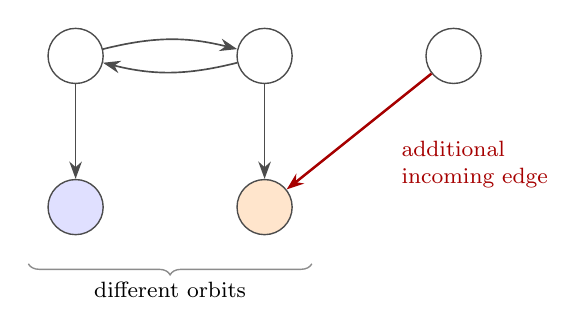
\begin{tikzpicture}[
  >={Stealth[length=2.2mm,width=1.6mm]},
  x=1.2cm, y=1.2cm,
]

\node[vtx]  (a) at (0.0, 1.6) {};
\node[vtx]  (b) at (2.0, 1.6) {};
\node[vtx]  (e) at (4.0, 1.6) {};
\node[orbA] (c) at (0.0, 0.0) {};
\node[orbB] (d) at (2.0, 0.0) {};

\draw[ed] (a) to[bend left=14] (b);
\draw[ed] (b) to[bend left=14] (a);

\draw[ed] (a) -- (c);
\draw[ed] (b) -- (d);

%% the edge that destroys the candidate automorphism c <-> d
\draw[edbreak] (e) -- (d);
\node[ann,anchor=west,align=left,text=red!65!black] at (3.4,0.45)
      {additional\\incoming edge};

\draw[decorate,decoration={brace,amplitude=4pt,mirror},draw=black!45,
      line width=0.5pt]
      (-0.5,-0.6) -- (2.5,-0.6)
      node[ann,midway,below=5pt] {different orbits};

\end{tikzpicture}
\caption{The symmetry of the two bottom nodes is broken by an incoming edge from elsewhere in the graph (all nodes carry the same label). Without the highlighted edge the two bottom nodes would be interchangeable; with it, no automorphism maps one onto the other, so they no longer lie in the same orbit. Their reachable subgraphs (a single sink each) are nevertheless identical, so any hash that looks only at reachable subgraphs must give them equal values.}
\label{fig:breaksymmetry}
\end{figure*}

In many real world applications the outgoing edges of each node are ordered. Examples include the links of a web page, the fields of a record, and the arguments of a function call. We take advantage of this extra structure to create simpler and faster hashing algorithms. The algorithms in this section were inspired by the more general Scott graph canonization algorithm of Bloyet, Marteau and Fr\'enod \cite{scott}. The basic idea is that, because the edges are ordered, a depth-first search from a given root visits the nodes in an order that is determined by the structure alone.

\paragraph{Model.} An \emph{ordered labeled digraph} assigns to each node $u$ a label $L(u)$ and a finite \emph{out-sequence} $s(u)=(s_1(u),\dots,s_{d(u)}(u))$ of successor nodes; position $k$ is the $k$-th \emph{port} of $u$, and repeated entries (two links to the same page) are allowed. An \emph{ordered isomorphism} $\phi:G_1\to G_2$ is a label-preserving bijection with $s(\phi(u)) = (\phi(s_1(u)),\dots,\phi(s_{d(u)}(u)))$ for all $u$. Ordered automorphisms, orbits and rooted ordered isomorphisms are defined accordingly. For a node $n$ we write $G[\Reach(n)]$ for the ordered subgraph induced on its reachable set.

\begin{exmp}[Edge order must be serialized]
\label{ex:ordered}
Sorting the relabeled adjacency list, as an earlier version of this algorithm did, loses the port order, and the depth-first numbering does not always recover it because edges to already-visited nodes do not affect the numbering. Take $s(r)=(x,y)$, $s(y)=()$, and either $s(x)=(y,r)$ or $s(x)=(r,y)$. In both graphs the search from $r$ numbers $r,x,y$ as $0,1,2$, and the sorted edge set is $\{(0,1),(0,2),(1,0),(1,2)\}$ in both cases, even though the two graphs are not ordered-isomorphic.
\end{exmp}

\begin{algorithm}[H]
    \caption{Node Hash --- Outgoing Ordered Edges}
    \label{alg:node-outgoing-edges}
    \begin{enumerate}
        \item From the input node $n$, perform a depth-first search that explores the out-edges of each node in port order, and number the reachable nodes $0,1,2,\dots$ in order of discovery (preorder).
        \item Create the list of original labels in discovery order.
        \item For each node in discovery order, write its out-sequence as a sequence of discovery numbers, \emph{keeping the port order} (do not sort).
        \item Return $\HO(G,n)=\mathcal{H}(\enc((\text{label list},\ \text{out-sequence list})))$.
    \end{enumerate}
\end{algorithm}

\begin{theorem}
\label{thm:orderedhash}
$\HO$ realizes rooted ordered isomorphism of reachable subgraphs: assuming $\mathcal{H}$ is injective, $\HO(G_1,n_1)=\HO(G_2,n_2)$ if and only if there is an ordered isomorphism $G_1[\Reach(n_1)]\to G_2[\Reach(n_2)]$ mapping $n_1$ to $n_2$. It runs in time $O(|\Reach(n)|+|E(\Reach(n))|)$ plus the cost of hashing.
\end{theorem}
\begin{proof}
($\Leftarrow$) The depth-first search is deterministic given the port orders. An ordered isomorphism $\psi$ commutes with every step of it: by induction on the steps, the searches from $n_1$ and $\psi(n_1)=n_2$ discover $x$ and $\psi(x)$ at the same step. Hence $\psi$ preserves discovery numbers, and the serializations coincide.
($\Rightarrow$) Equal serializations have equal lengths. Map the $k$-th discovered node of $G_1$ to the $k$-th discovered node of $G_2$. The label lists agree, and the out-sequences of corresponding nodes are equal as sequences of discovery numbers, so the map is an ordered isomorphism mapping $n_1$ (number $0$) to $n_2$.
\end{proof}

$\HO$ is a hash of the reachable subgraph, not of the unfolding. For example, a node with a self-loop and a node on a 2-cycle (with all labels equal) have isomorphic unfoldings but different values of $\HO$. The local, unfolding-based notion is easier in the ordered setting than in Section~\ref{sec:local-graph-hashing}, because an ordered graph is a deterministic automaton whose input letters are ports and whose output at each state is the pair (label, out-degree).

\begin{prop}[Ordered local hashing]
\label{prop:ordered-local}
Refine with sequences in place of multisets, $\lambda_{i+1}(u)=\mathcal{H}(\enc((L(u),(\lambda_i(s_1(u)),\dots,\lambda_i(s_{d(u)}(u))))))$, until global stabilization, and form the quotient $Q$ with $s([u]) = ([s_1(u)],\dots,[s_{d(u)}(u)])$. Then $u\mapsto\HO(Q,[u])$ realizes isomorphism of ordered unfoldings. The quotient is the minimal automaton, and it can be computed in $O(m\log n)$ time with partial-DFA minimization \cite{hopcraft,valmari2008partial}.
\end{prop}
\begin{proof}[Proof sketch]
As in Lemmas~\ref{lem:colors-trunc}--\ref{lem:quotient}, the stable classes are exactly the ordered-unfolding classes, the quotient is well defined and preserves ordered unfoldings, and distinct vertices of $Q$ have distinct ordered unfoldings. If $\Unf(G_1,u)\iso\Unf(G_2,v)$ as ordered trees, then the simultaneous traversal of $Q_1$ from $[u]$ and $Q_2$ from $[v]$ along equal ports reaches vertices with isomorphic ordered unfoldings. By minimality this defines a bijection between the reachable sets, which is an ordered isomorphism, so Theorem~\ref{thm:orderedhash} applies. The converse is as in Theorem~\ref{thm:localhashcorrect}.
\end{proof}

\paragraph{Strongly connected graphs.} For the special case of a strongly connected ordered graph, the node hashes of Algorithm~\ref{alg:node-outgoing-edges} yield both a canonical form and the orbit partition in polynomial time. This is the case needed by the Merkle-style hashing of Section~\ref{sec:merkle-graph-hashing}, where strongly connected components are hashed individually.

\begin{algorithm}[H]
    \caption{Canonization and Orbit Partitioning for Strongly Connected Ordered Graphs}
    \label{alg:scc-outgoing-edges}
    \begin{enumerate}
        \item For each node $n$, compute $\HO(G,n)$ using Algorithm \ref{alg:node-outgoing-edges}. The orbits are the classes of equal $\HO$ values.
        \item Choose any node $r$ with minimal $\HO$ value. Its discovery order is the canonical labeling $\rho$, and its serialization is the canonical form $\canon(G)$.
        \item The graph hash is $\mathcal{H}(\enc(\canon(G)))$, and the orbit index of $v$ is $\min\{\rho(x)\mid \HO(G,x)=\HO(G,v)\}$. These are used exactly as in Algorithm~\ref{alg:digraph-node-hash}.
    \end{enumerate}
\end{algorithm}

\begin{theorem}
\label{thm:scc-ordered}
Let $G_1,G_2$ be strongly connected ordered digraphs with $n$ nodes and $m$ edges, and assume $\mathcal{H}$ is injective. Then:
(a) $\HO(G_1,u)=\HO(G_2,v)$ if and only if there is an ordered isomorphism $\phi:G_1\to G_2$ with $\phi(u)=v$; in particular, the classes of Step~1 are exactly the orbits;
(b) $\canon(G_1)=\canon(G_2)$ if and only if $G_1\iso G_2$, and $\rho$ is an isomorphism onto $\canon(G)$;
(c) the node hash of Step~3 realizes rooted ordered isomorphism, as in Theorem~\ref{thm:digraphnodehashcorrect};
(d) every ordered automorphism is determined by the image of a single node, so $|\Aut(G)|\le n$ and all orbits have equal size;
(e) Algorithm~\ref{alg:scc-outgoing-edges} runs in $O(n(n+m))$ time plus the cost of hashing.
\end{theorem}
\begin{proof}
(a) Since $G_i$ is strongly connected, $\Reach(u)=V_1$ and $\Reach(v)=V_2$, so this is Theorem~\ref{thm:orderedhash}.
(b) If $\phi : G_1 \to G_2$ is an isomorphism, then by (a) $\phi$ maps nodes to nodes with equal $\HO$ values. The minimal values therefore coincide, and all minimizing nodes have the same serialization, which is determined by the hash. Conversely, equal serializations yield an isomorphism as in Theorem~\ref{thm:orderedhash}. The discovery order is exactly the bijection onto the serialized graph.
(c) With (b) in place of the canonizer, the proof of Theorem~\ref{thm:digraphnodehashcorrect} applies verbatim; the orbit index of Step~3 is the minimum canonical index over the orbit by (a).
(d) An automorphism commutes with the depth-first search from any node $u$, which reaches all nodes, so it is determined by $\sigma(u)$. Hence $\Aut(G)$ acts semiregularly.
(e) The algorithm runs $n$ searches of cost $O(n+m)$ each.
\end{proof}

\paragraph{Why only strongly connected graphs?} For a general digraph, the orbit of a node depends not only on the structure of its reachable subgraph but also on its ancestors. Incoming edges can break the symmetry of an orbit, as demonstrated in Figure \ref{fig:breaksymmetry}, so the reachable-subgraph hashes of Algorithm~\ref{alg:node-outgoing-edges} can be equal for nodes in different orbits. In a strongly connected graph this cannot happen, because every node reaches every other node. We do not address canonization of general (not strongly connected) ordered digraphs here, as the Merkle construction below only needs strongly connected components.

\section{Merkle Graph Hashing}
\label{sec:merkle-graph-hashing}

For applications where graphs are built up over time, a recursive approach similar to Merkle-tree hashing is highly beneficial. We now construct such an algorithm, which recurses over the condensation graph. The condensation is acyclic, so the recursion is well founded.

To compute the hash of each node, we process the strongly connected components in reverse topological order, so that every edge leaving a component points to nodes that have already been hashed. Each node of the component is relabeled by combining its label with the hashes of its external targets: a multiset of hashes for unordered graphs; for ordered graphs, the out-sequence in which every internal target is replaced by a placeholder $\star$, so that the positions of internal and external links are both recorded. Finally the relabeled component, restricted to its internal edges, is hashed with the global node hash (Algorithm~\ref{alg:digraph-node-hash}) or, for ordered graphs, with Algorithm~\ref{alg:scc-outgoing-edges}. Algorithm \ref{alg:merklegraphhash} gives the pseudo-code; each component is processed once.

\begin{algorithm}
    \caption{Merkle Graph Node Hashing}\label{alg:merklegraphhash}
    \begin{algorithmic}[1]
    \Function{$\HM$}{$G=(V,E,L)$}
        \State $h \gets \textproc{empty\_dict}()$
        \For{\textbf{each} SCC $S$ in reverse topological order} \Comment{Tarjan's algorithm; sinks first}
          \For{$x \in S$}
            \If{outgoing edges are unordered}
              \State $X(x) \gets \mset{h[y] \mid y\notin S \land (x,y)\in E}$
            \Else
              \State $X(x) \gets (\,h[y] \text{ if } y\notin S \text{ else } \star \mid y \in s(x)\,)$
            \EndIf
            \State $L'(x) \gets \mathcal{H}(\enc((L(x), X(x))))$
          \EndFor
          \State $G' \gets (S,\ E\cap (S\times S),\ L')$ \Comment{ordered case: keep internal targets in port order}
          \For{$x \in S$}
            \State $h[x] \gets \HN(G', x)$ \Comment{ordered case: node hash of Algorithm~\ref{alg:scc-outgoing-edges}}
          \EndFor
        \EndFor
        \State \Return $h$
    \EndFunction
    \end{algorithmic}
\end{algorithm}

Which nodes receive equal hashes? Within a component the hash is global (it respects automorphisms, including incoming edges inside the component), while across components it behaves like a Merkle tree: it compares external targets only through their hashes and ignores whether two targets are shared. We make this precise. For a node $u$ let $S(u)$ denote its SCC.

\begin{defn}[Merkle equivalence]
\label{def:merkle-eq}
For nodes $u$ of $G_1$ and $v$ of $G_2$, define $u\approx_M v$ by well-founded recursion on the heights of $S(u)$ and $S(v)$: $u\approx_M v$ if and only if there is a bijection $\phi:S(u)\to S(v)$ with $\phi(u)=v$ such that, for every $x\in S(u)$,
\begin{enumerate}[label=(\roman*)]
  \item $L_1(x)=L_2(\phi(x))$, and $\phi$ is an isomorphism of the subgraphs induced on $S(u)$ and $S(v)$;
  \item there is a bijection between the external successors of $x$ and those of $\phi(x)$ that relates only $\approx_M$-equivalent nodes.
\end{enumerate}
In the ordered variant, (i) and (ii) are replaced by: $L_1(x)=L_2(\phi(x))$, $d(x)=d(\phi(x))$, and for every port $k$, either both $s_k(x)\in S(u)$ and $s_k(\phi(x))=\phi(s_k(x))$, or both targets are external and $s_k(x)\approx_M s_k(\phi(x))$.
\end{defn}

The recursion is well founded because external successors lie in SCCs of strictly smaller height. By induction on height, $\approx_M$ is an equivalence relation.

\begin{theorem}[Correctness of the Merkle hash]
\label{thm:merkle}
$\HM$ realizes $\approx_M$ (in both variants): assuming $\mathcal{H}$ is injective, $\HM(G_1)[u]=\HM(G_2)[v]$ if and only if $u\approx_M v$.
\end{theorem}
\begin{proof}
By induction on the maximum of the heights of $S(u)$ and $S(v)$. By the induction hypothesis (and trivially at height $0$, where there are no external successors), for $x\in S(u)$ and $y\in S(v)$ the multisets (respectively, $\star$-masked sequences) $X(x)$ and $X(y)$ are equal if and only if the external successors of $x$ and $y$ can be matched by $\approx_M$ (respectively, port by port). Hence $L'(x)=L'(y)$ if and only if $L(x)=L(y)$ and condition (ii) holds. Now apply Theorem~\ref{thm:digraphnodehashcorrect} (respectively, Theorem~\ref{thm:scc-ordered}(c)) to the relabeled components: the node hashes are equal if and only if there is an $L'$-preserving isomorphism of the relabeled components mapping $u$ to $v$. In the ordered case the isomorphism must also preserve the order of internal targets, and together with the $\star$-masks this means preserving each port. This is exactly Definition~\ref{def:merkle-eq}.
\end{proof}

\begin{prop}
\label{prop:merkle-position}
For nodes $u$ of $G_1$ and $v$ of $G_2$: if $(G_1[\Reach(u)],u)\iso(G_2[\Reach(v)],v)$ then $u\approx_M v$, and if $u\approx_M v$ then $\Unf(G_1,u)\iso\Unf(G_2,v)$. Neither converse holds. The same statements hold in the ordered setting.
\end{prop}
\begin{proof}
A rooted isomorphism of reachable subgraphs maps SCCs to SCCs, so it witnesses Definition~\ref{def:merkle-eq} at every level. For the second implication, proceed by induction on height. A walk from $u$ stays in $S(u)$ for a while and may then leave it along an external edge $x\to y$. Map the part inside $S(u)$ step by step with $\phi$, and at the exit edge use the bijection of condition (ii) to pair $y$ with some $y'\approx_M y$, whose unfoldings are isomorphic by induction. This assembles an isomorphism of the unfoldings.

For strictness of the first implication, let $x\to p$, $x\to q$, $p\to s$ and $q\to s$ (with $p,q$ equally labeled), and compare with the same graph in which $s$ is replaced by two copies $s_1,s_2$ with $p\to s_1$ and $q\to s_2$. The nodes $x$ are $\approx_M$-equivalent, since all SCCs are singletons and the external multisets agree, but the reachable subgraphs have $4$ and $5$ nodes. For strictness of the second, a node with a self-loop and a node on a $2$-cycle (all labels equal) have isomorphic unfoldings but are not $\approx_M$-equivalent, since their SCCs have different sizes.
\end{proof}

Thus the Merkle hash deliberately forgets whether subgraphs below a component are shared, exactly as Merkle trees and Merkle DAGs do in git and IPFS, while retaining full global structure inside each cycle.

\paragraph{Complexity and incrementality.} Computing the SCCs takes $O(n+m)$ time, and each component is hashed once. The total cost is $O(n+m)$ plus $\sum_S c(S)$, where $c(S)$ is the cost of Algorithm~\ref{alg:digraph-node-hash} on $S$ (GI-hard in general) or of Algorithm~\ref{alg:scc-outgoing-edges}, $O(|S|(|S|+m_S))$, in the ordered case. As with Merkle trees, changing a node changes only the hashes of nodes from which it is reachable. Adding a new node whose edges point only to existing nodes creates a new singleton SCC and leaves all existing hashes unchanged.

\section{Application Sketch}
\label{sec:application}

\begin{figure*}
\centering

% Row 1: Original HTML snippets
\textbf{Row 1: Original HTML Pages}

\vspace{0.15cm}

\begin{adjustbox}{max width=\textwidth}
\begin{tabular}{p{5.5cm}@{\hspace{0.3cm}}p{5.5cm}@{\hspace{0.3cm}}p{5.5cm}}
index.html
\begin{lstlisting}[language=HTML]
<body>
 <h1>Welcome</h1>
 <a href="about.html">
  About Us
 </a>
 <a href="http://e.com">
  External Resource
 </a>
</body>
\end{lstlisting}
&
about.html
\begin{lstlisting}[language=HTML]
<body>
 <h1>About Us</h1>
 <a href="index.html">
  Home
 </a>
 <a href="contact.html">
  Contact
 </a>
 <a href="http://p.com">
  Partner Site
 </a>
</body>
\end{lstlisting}
&
contact.html
\begin{lstlisting}[language=HTML]
<body>
 <h1>Contact Us</h1>
 <a href="about.html">
  About
 </a>
 <a href="http://e.com">
  External Resource
 </a>
</body>
\end{lstlisting}
\end{tabular}
\end{adjustbox}

\vspace{0.15cm}

% Row 2: Tokenized/Hashed HTML snippets
\textbf{Row 2: Replace intra-SCC links with their internal port numbers, and inter-SCC links with recursively computed hashes}

\vspace{0.15cm}

\begin{adjustbox}{max width=\textwidth}
\begin{tabular}{p{5.5cm}@{\hspace{0.3cm}}p{5.5cm}@{\hspace{0.3cm}}p{5.5cm}}
index.html
\begin{lstlisting}[language=HTML]
<body>
 <h1>Welcome</h1>
 <a href="{0}">
  About Us
 </a>
 <a href="#8ab43f">
  External Resource
 </a>
</body>
\end{lstlisting}
&
about.html
\begin{lstlisting}[language=HTML]
<body>
 <h1>About Us</h1>
 <a href="{0}">
  Home
 </a>
 <a href="{1}">
  Contact
 </a>
 <a href="#f2d91c">
  Partner Site
 </a>
</body>
\end{lstlisting}
&
contact.html
\begin{lstlisting}[language=HTML]
<body>
 <h1>Contact Us</h1>
 <a href="{0}">
  About
 </a>
 <a href="#8ab43f">
  External Resource
 </a>
</body>
\end{lstlisting}
\end{tabular}
\end{adjustbox}

\vspace{0.15cm}

% Row 3: Graph representation
\textbf{Row 3: Construct strongly connected ordered digraph (labels taken from previous row)}

\vspace{0.15cm}

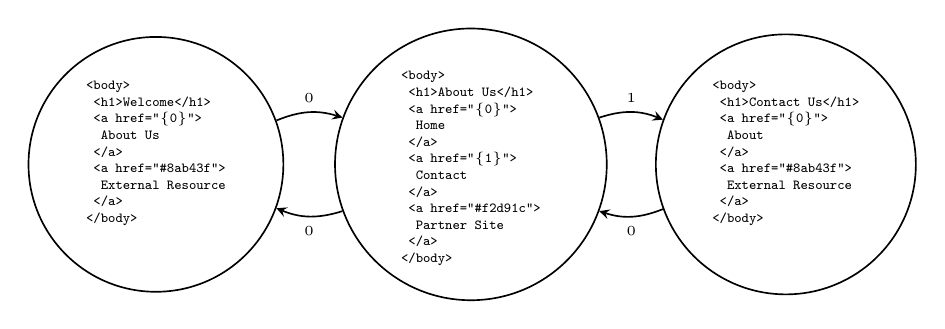
\begin{tikzpicture}[
    > = stealth, % arrow head style
    node distance=4cm,
    every node/.style={draw, align=left, font=\tiny},
    semithick % line style
]

% Nodes
\node[state] (index) {\\ \texttt{<body>} \\ \texttt{ <h1>Welcome</h1>} \\ \texttt{ <a href="\{0\}">} \\ \texttt{ ~About Us} \\ \texttt{ </a>} \\ \texttt{ <a href="\#8ab43f">} \\ \texttt{ ~External Resource} \\ \texttt{ </a>} \\ \texttt{</body>} \\ \\};
\node[state] (about) [right of=index] { \\ \texttt{<body>} \\ \texttt{ <h1>About Us</h1>} \\ \texttt{ <a href="\{0\}">} \\ \texttt{ ~Home} \\ \texttt{ </a>} \\ \texttt{ <a href="\{1\}">} \\ \texttt{ ~Contact} \\ \texttt{ </a>} \\ \texttt{ <a href="\#f2d91c">} \\ \texttt{ ~Partner Site} \\ \texttt{ </a>} \\ \texttt{</body>}};
\node[state] (contact) [right of= about] {\\ \texttt{<body>} \\ \texttt{ <h1>Contact Us</h1>} \\ \texttt{ <a href="\{0\}">} \\ \texttt{ ~About} \\ \texttt{ </a>} \\ \texttt{ <a href="\#8ab43f">} \\ \texttt{ ~External Resource} \\ \texttt{ </a>} \\ \texttt{</body>} \\ \\};

% Edges (internal links only), labelled by internal port number
\draw[->] (index) to[bend left=20] node[above, draw=none] {0} (about);
\draw[->] (about) to[bend left=20] node[below, draw=none] {0} (index);
\draw[->] (about) to[bend left=20] node[above, draw=none] {1} (contact);
\draw[->] (contact) to[bend left=20] node[below, draw=none] {0} (about);

\end{tikzpicture}

\caption{Hashing a three page website that forms a single SCC. In Row 2, \texttt{\{k\}} marks a page's $k$-th intra-SCC link (the placeholder $\star$ of Algorithm~\ref{alg:merklegraphhash}), and \#8ab43f, \#f2d91c are recursively computed hashes of external pages.}
\label{fig:webpage-example}
\end{figure*}

From the algorithms given so far, it may not be obvious how to implement these graph theoretic procedures for real world data. Here we show how to do so for a static hyperlinked web page system stored in a content addressed distributed hash table (DHT).

In this sketch, we assume that web pages are static HTML files that link to each other and to external pages, and that external pages are themselves published in the same content-addressed way. (An external page that links back into our site would belong to the same SCC and be hashed together with it.) The pages form an ordered digraph in which each page is a node, the links are edges, and the out-edges of a node are ordered by their position in the HTML file. Figure \ref{fig:webpage-example} gives a concrete example of the process described here.

We first compute the SCCs of the link graph and process them sinks first, as in Algorithm~\ref{alg:merklegraphhash}. Within a page, every link to another page of the same SCC is replaced by its internal port number, and every link leaving the SCC is replaced by the recursively computed hash of its target. The resulting text is the relabeled node label $L'$ of the ordered variant. We then compute the canonical labeling, canonical form and orbit partition of the SCC in $O(n(n+m))$ time using Algorithm \ref{alg:scc-outgoing-edges}, and insert the following items into the distributed hash table:

\begin{itemize}
  \item The strongly connected component as a whole: \begin{itemize}
    \item \textbf{Value}: the canonical form, i.e.\ the list of relabeled page contents in canonical order together with each page's internal out-sequence in canonical indices.
    \item \textbf{Key}: the string hash $\mathcal{H}$ of the value.
  \end{itemize}
  \item For each page, a reference to a specific node in the strongly connected component: \begin{itemize}
    \item \textbf{Value}: the orbit index of the page, together with the key of its SCC.
    \item \textbf{Key}: the string hash $\mathcal{H}$ of the value. This is the page's hash.
  \end{itemize}
\end{itemize}

By Theorem~\ref{thm:merkle}, two pages receive the same key exactly when they are $\approx_M$-equivalent. In particular, pages in the same orbit of an SCC share a key. This is harmless, since such pages are indistinguishable by any navigation.

Suppose that a user wants to navigate our website and has obtained the hash of one specific page. The browser retrieves the orbit index and SCC key from the DHT, then retrieves the SCC itself, which allows the SCC digraph to be reconstructed. The orbit index points to a specific node of the canonical form, whose contents the browser displays. If the user clicks a link within the same SCC, the browser follows the corresponding internal edge. For links that leave the SCC, the embedded hash is a page key, and the browser repeats the process from the beginning. As with any Merkle structure, editing a page changes the keys of that page's SCC and of all pages from which it can be reached, and of no others.

\section{Related Work}
\label{sec:related}

\paragraph{Merkle hashing of cyclic definitions.} The core idea of the digraph Merkle hashing algorithm was independently discovered by the developers of the Unison programming language \cite{unison}, who hash the abstract syntax trees of mutually recursive definitions. Each function and datatype is a node in a digraph, with its AST as the node label, and each cycle of mutually recursive definitions is hashed as a unit. To our knowledge their scheme does not treat non-trivial automorphism orbits inside a cycle, which arise, for example, from two structurally identical mutually recursive definitions that differ only in name. Such orbits appear to be rare in practice, but a complete treatment requires the orbit index of Algorithm~\ref{alg:digraph-node-hash}. Hash-consing of cyclic structures and unique representations of regular trees \cite{mauborgne2000incremental}, as well as hashing of terms modulo $\alpha$-equivalence \cite{maziarz2021hashing}, address closely related problems in programming language implementation.

\paragraph{Color refinement and Weisfeiler--Leman.} The Weisfeiler--Lehman graph hash \cite{Shervashidze2011-dt} iteratively hashes and aggregates the neighborhoods of each node of an undirected graph. Isomorphic graphs are guaranteed to receive equal hashes, but the converse fails: 1-dimensional Weisfeiler--Leman refinement \cite{weisfeiler1968reduction} cannot distinguish, for example, two disjoint triangles from a $6$-cycle, or any two regular graphs of the same order and degree. In the kernel literature the number of iterations $h$ is a parameter that controls the depth of the subtree features. When refinement is used to test or hash equivalence, as here, no parameter is needed, because the partition stabilizes within $n-1$ rounds (Lemma~\ref{thm:stability}). Efficient implementations of color refinement run in $O((n+m)\log n)$ time \cite{cardon1982partitioning,berkholz2017tight}. The algorithm of Section \ref{sec:local-graph-hashing} is a directed, canonical variant of the Weisfeiler--Lehman hash. The equivalence it computes is the view equivalence of anonymous networks \cite{yamashita1996anonymous} and the fibration equivalence of Boldi and Vigna \cite{boldi2002fibrations}, and for undirected graphs it corresponds to isomorphism of universal covers \cite{norris1995universal}.

\paragraph{Bisimulation and automata.} Bisimilarity is computed by relational coarsest partition algorithms \cite{kanellakis1990ccs,paige1987three}, and state equivalence of deterministic automata by Hopcroft-style minimization \cite{hopcraft,hopcraft-redescribe,valmari2008partial}. Sections~\ref{sec:local-graph-hashing} and \ref{sec:outgoing-ordered-edge-graphs} use these as the first stage of canonical hashing.

\paragraph{Canonization.} Canonical labeling tools \cite{nauty,mckay2014practical,bliss,saucy} and Babai's quasipolynomial-time isomorphism test and canonization \cite{babai2016quasipolynomial,babai2019canonical} underlie Section~\ref{sec:global-graph-hashing}.

\paragraph{Arshad et al.} In a 2014 paper, Arshad et al. \cite{Arshad2014-cc} presented an algorithm for hashing directed graphs given additional inputs: a fixed source node and a depth-first search traversal tree. The traversal tree classifies the edges as tree, back, forward, and cross edges depending on search order, and the hash uses the traversal numbers to order the nodes. The authors note that isomorphic graphs may hash to different values because of this dependence on the source node and DFS tree. Their approach can be used to hash nodes with ordered outgoing edges and can be viewed as an alternative to Algorithm~\ref{alg:node-outgoing-edges}.

In a separate 2018 paper, Arshad et al. \cite{Arshad2018-ij} presented a graph hashing algorithm in which the hash of a node combines, by XOR, the hashes of the labels of all of that node's descendants; the graph hash is then computed by hashing each node together with an accumulated graph hash. As described, this approach has two weaknesses. First, XOR aggregation is not a multiset hash: an even number of identically labeled descendants cancels out, so a node with two identically labeled descendants contributes as if it had none. Second, the aggregation ignores the edge structure among the descendants. For example, in the directed $k$-cycle and in the complete digraph on $k$ vertices, with all labels equal, every node has the same $k-1$ identically labeled descendants, so the algorithm outputs equal hashes for these non-isomorphic graphs.

\section{Experimental Results}
\label{sec:experiments}

We implemented all algorithms of this paper in Python 3.11 as an exact reference implementation, using SHA-256 over a length-prefixed injective encoding. Global canonization uses a simple exhaustive individualization-refinement search, adequate for small graphs. Running times were measured on a single core of an Intel Xeon processor at 2.8\,GHz. The implementation is intended to validate the theorems, not to compete with optimized tools.

\paragraph{Validation.} We generated 1000 pairs of random labeled digraphs with 1--6 nodes each (edge probability $0.15$, $0.3$ or $0.5$, self-loops allowed, one or two labels). In half of the pairs the second graph is a random relabeling of the first. For every pair of nodes we compared hash equality with an independent brute-force decision of the corresponding equivalence:
\begin{itemize}
  \item isomorphism and rooted isomorphism, by enumerating all bijections;
  \item unfolding isomorphism, by comparing canonical forms of truncated unfoldings of depth $n_1+n_2+1$;
  \item bisimilarity, by a greatest-fixpoint computation;
  \item rooted ordered isomorphism, by simultaneous traversal.
\end{itemize}
For $\approx_M$ we used a direct implementation of Definition~\ref{def:merkle-eq}. We also tested the ordered orbit partition of Theorem~\ref{thm:scc-ordered} against brute-force search on every SCC. Table~\ref{tab:validation} summarizes the results. No disagreement was found. The same harness confirms the counterexamples of Examples~\ref{ex:bisim} and~\ref{ex:ordered} for the naive variants, and the orbit structure claimed in Figure~\ref{fig:orbitexample}.

\begin{table}[t]
\centering
\caption{Validation against brute-force equivalence checks: number of node pairs (or SCCs) compared, with no disagreements in any row.}
\label{tab:validation}
\begin{tabular}{@{}lr@{}}
\toprule
Scheme (theorem) & Pairs checked \\
\midrule
Global graph hash (Thm.~\ref{thm:digraphhashcorrect}) & 1{,}000 graphs \\
Global node hash (Thm.~\ref{thm:digraphnodehashcorrect}) & 12{,}947 \\
Local hash (Thm.~\ref{thm:localhashcorrect}) & 12{,}947 \\
Bisimulation hash (Thm.~\ref{thm:bisimhash}) & 12{,}947 \\
Ordered node hash (Thm.~\ref{thm:orderedhash}) & 12{,}720 \\
Ordered local hash (Prop.~\ref{prop:ordered-local}) & 12{,}720 \\
Ordered SCC orbits (Thm.~\ref{thm:scc-ordered}) & 2{,}487 SCCs \\
Merkle hash, both variants (Thm.~\ref{thm:merkle}) & 26{,}794 \\
\bottomrule
\end{tabular}
\end{table}

\paragraph{Scaling.} Table~\ref{tab:scaling} reports median running times over three random ordered digraphs per size, with two labels and $2n$ randomly drawn edges (duplicates discarded; average out-degree just under $2$). These graphs have a giant strongly connected component containing 60--65\% of the nodes. Global stabilization was detected after 5--6 refinement rounds at all sizes. The time to hash all nodes grows roughly by a factor of four each time $n$ doubles, i.e.\ quadratically. This matches the output-sensitive term $\sum_x |\Reach(x)|$ discussed in Section~\ref{sec:local-graph-hashing}: most nodes reach the giant component. The cubic worst case is not attained because few rounds are needed. The Merkle hash is cheaper than hashing every node with $\HO$ because the DFS-based work is confined to each SCC, with external targets summarized by their hashes.

\begin{table}[t]
\centering
\caption{Median time in seconds to hash all nodes of a random ordered digraph with $n$ nodes and $2n$ edges (Python prototype).}
\label{tab:scaling}
\begin{tabular}{@{}rrrrrrr@{}}
\toprule
$n$ & largest SCC & $\HL$ & $\HB$ & $\HO$ & ordered local & $\HM$ (ordered) \\
\midrule
250  & 151  & 0.26  & 0.21  & 0.11 & 0.11 & 0.08 \\
500  & 314  & 1.07  & 0.94  & 0.51 & 0.41 & 0.36 \\
1000 & 646  & 4.43  & 3.90  & 2.00 & 1.84 & 1.27 \\
2000 & 1272 & 19.80 & 16.73 & 7.99 & 6.90 & 5.45 \\
\bottomrule
\end{tabular}
\end{table}

\paragraph{Granularity.} To illustrate how the equivalences compare, we hashed 400 random unlabeled digraphs with 12 nodes and 18 randomly drawn edges (duplicates discarded) and counted the distinct hash values per graph. On average the graphs have 12 nodes and 11.82 orbits (global node hash). They have 9.81 $\approx_M$ classes (Merkle hash), 9.13 unfolding classes (local hash), and 7.76 bisimulation classes. This is consistent with the implications rooted isomorphism $\Rightarrow$ $\approx_M$ $\Rightarrow$ unfolding isomorphism $\Rightarrow$ bisimilarity (Proposition~\ref{prop:merkle-position} and Section~\ref{sec:local-graph-hashing}). The gaps show that the choice of equivalence matters in practice even on small random graphs.

\section{Conclusion}
\label{sec:conclusion}

We have given hashing schemes for node-labeled digraphs whose hash equality corresponds exactly, up to collisions of the underlying string hash, to isomorphism, rooted isomorphism, unfolding isomorphism, bisimilarity, and a Merkle-style equivalence, together with fast variants for graphs with ordered outgoing edges. Natural directions for future work include an $O((n+m)\log n)$ implementation of the local stage via partition refinement, output-sensitive or incremental computation of local hashes, polynomial canonization of general ordered digraphs, and evaluation on real data such as version-control object graphs and web crawls.

% SIAM recommends using BibTeX
\bibliographystyle{siamplain}
\bibliography{example_references,dihash_additional_references}

\end{document}
